\begin{figure}
        \centering
        \begin{subfigure}[b]{0.5\textwidth}
                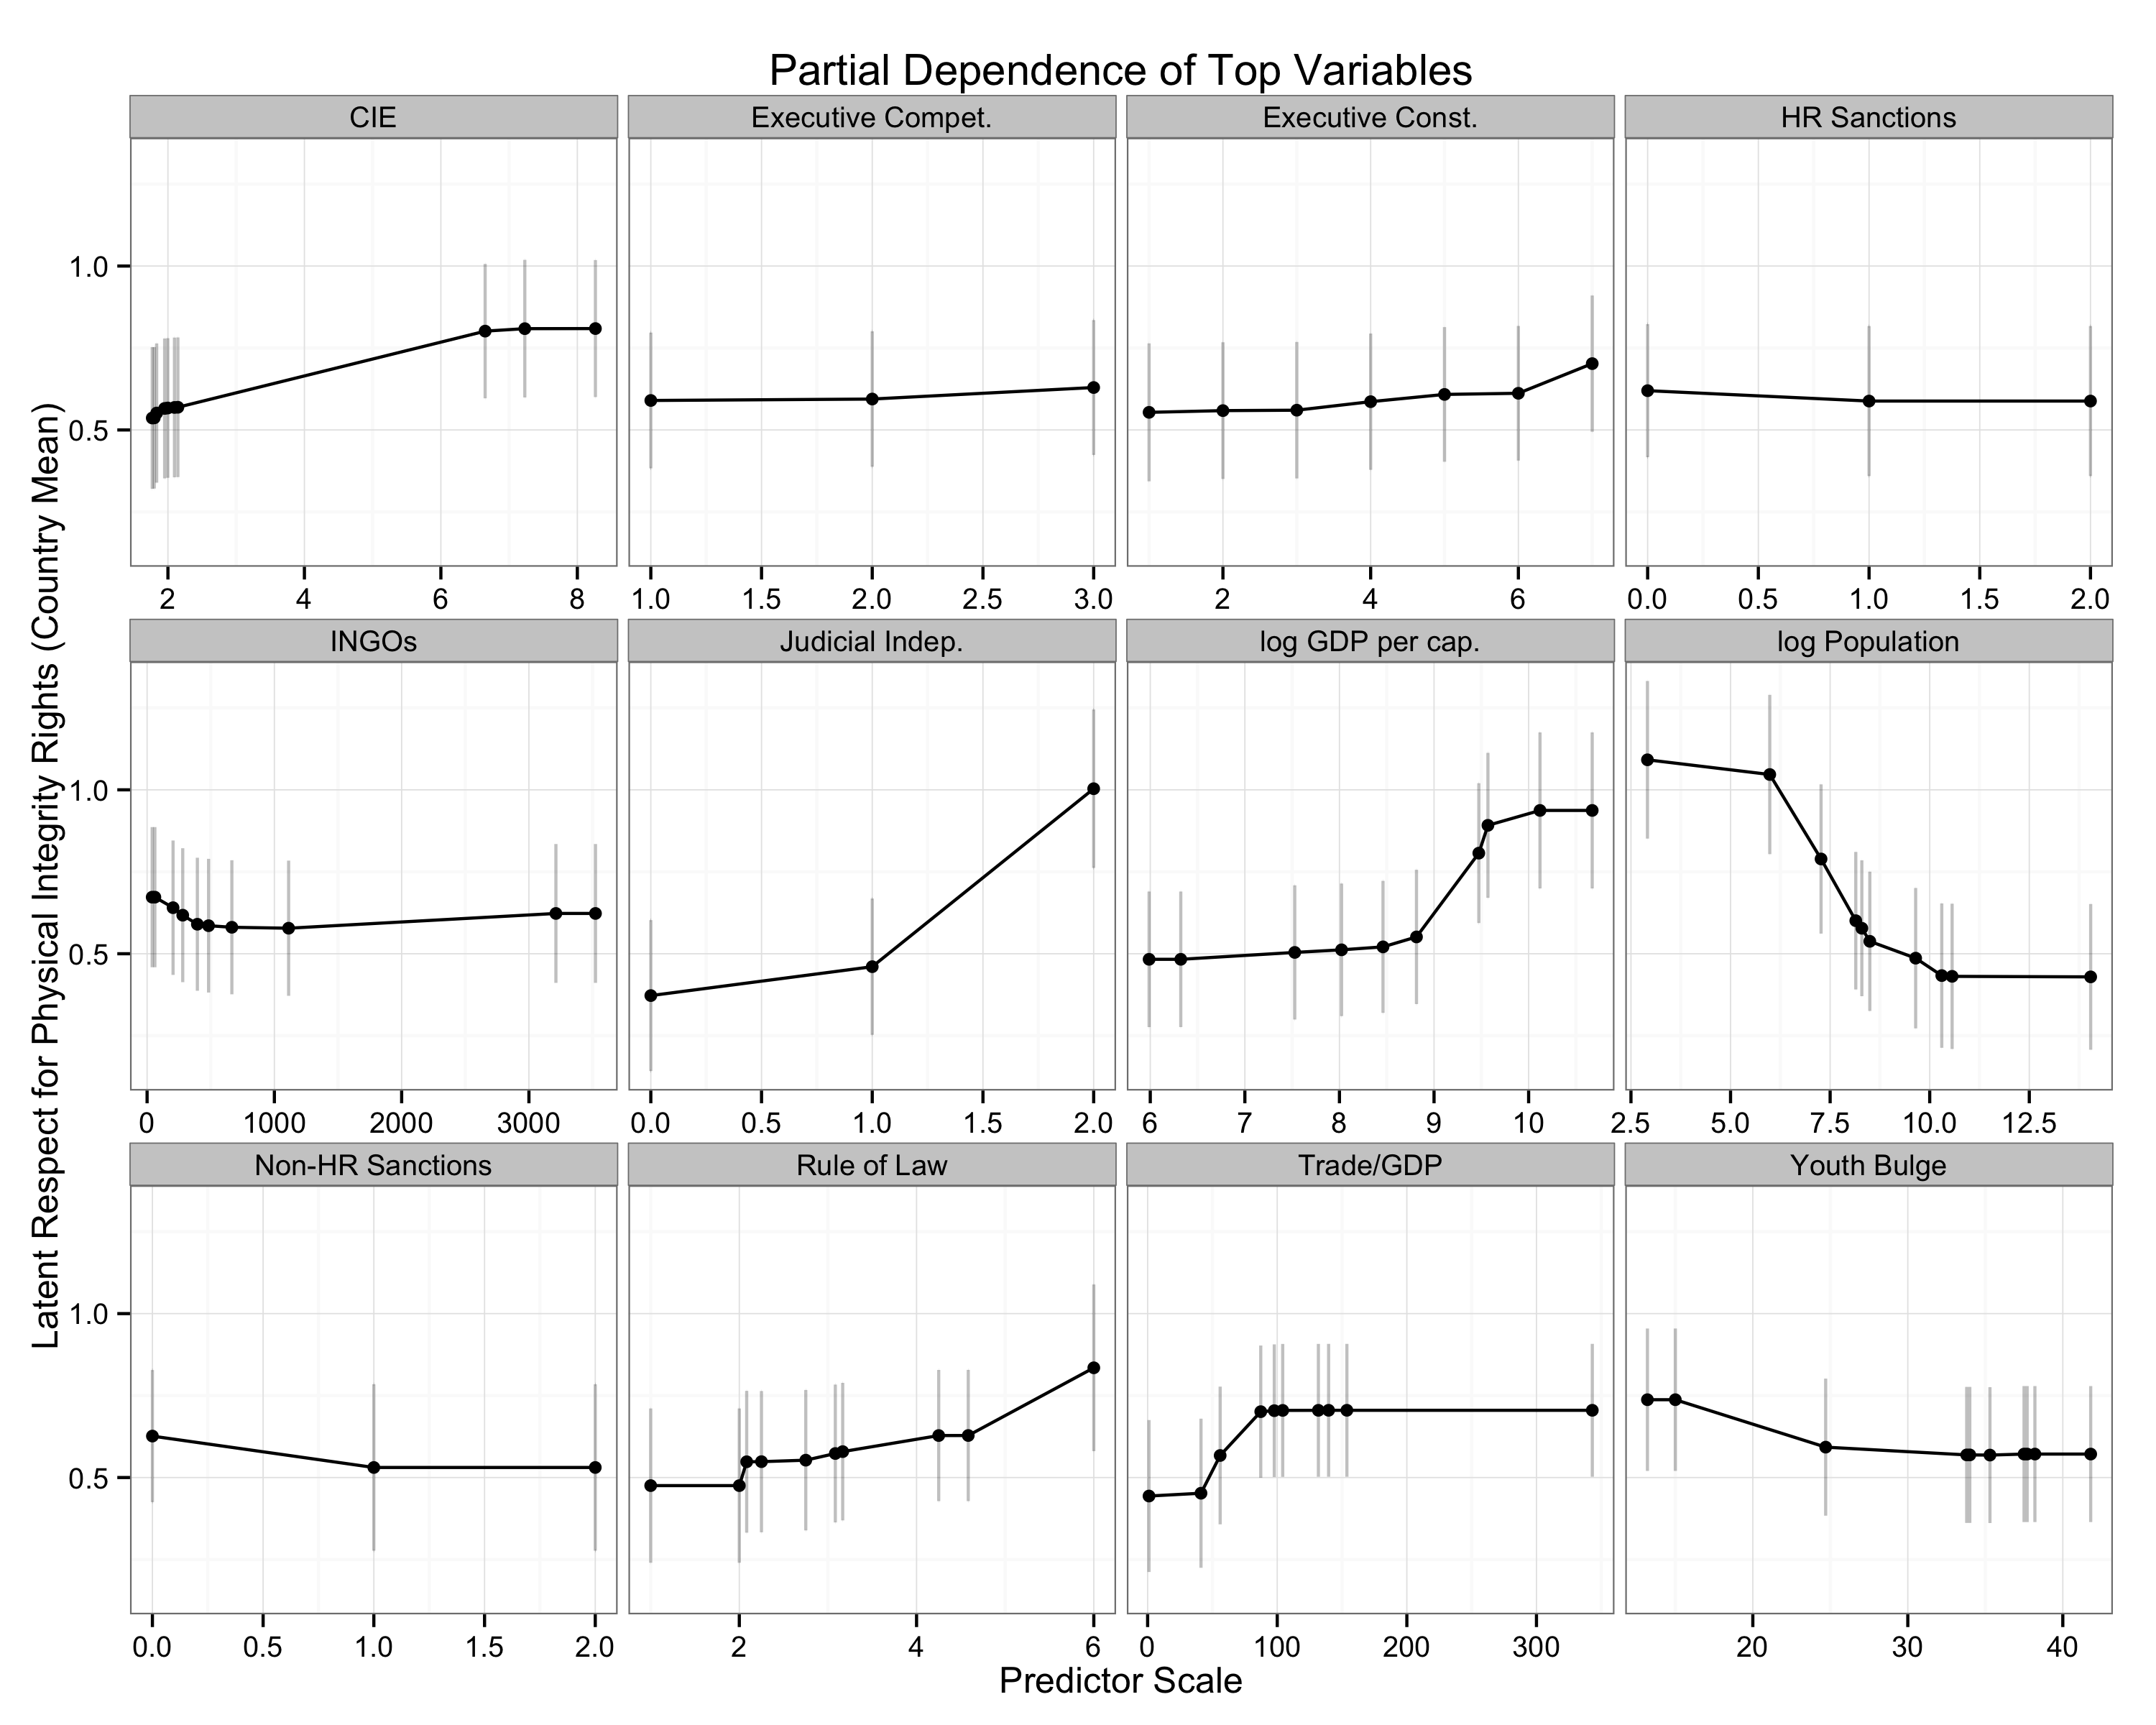
\includegraphics[width=\textwidth]{figures/latent_pd.png}
                \caption{Partial dependence for predictors of latent respect for human rights.}
                \label{fig:latent_pd}
        \end{subfigure}%
        ~ %add desired spacing between images, e. g. ~, \quad, \qquad, \hfill etc.
          %(or a blank line to force the subfigure onto a new line)

        \begin{subfigure}[b]{0.5\textwidth}
                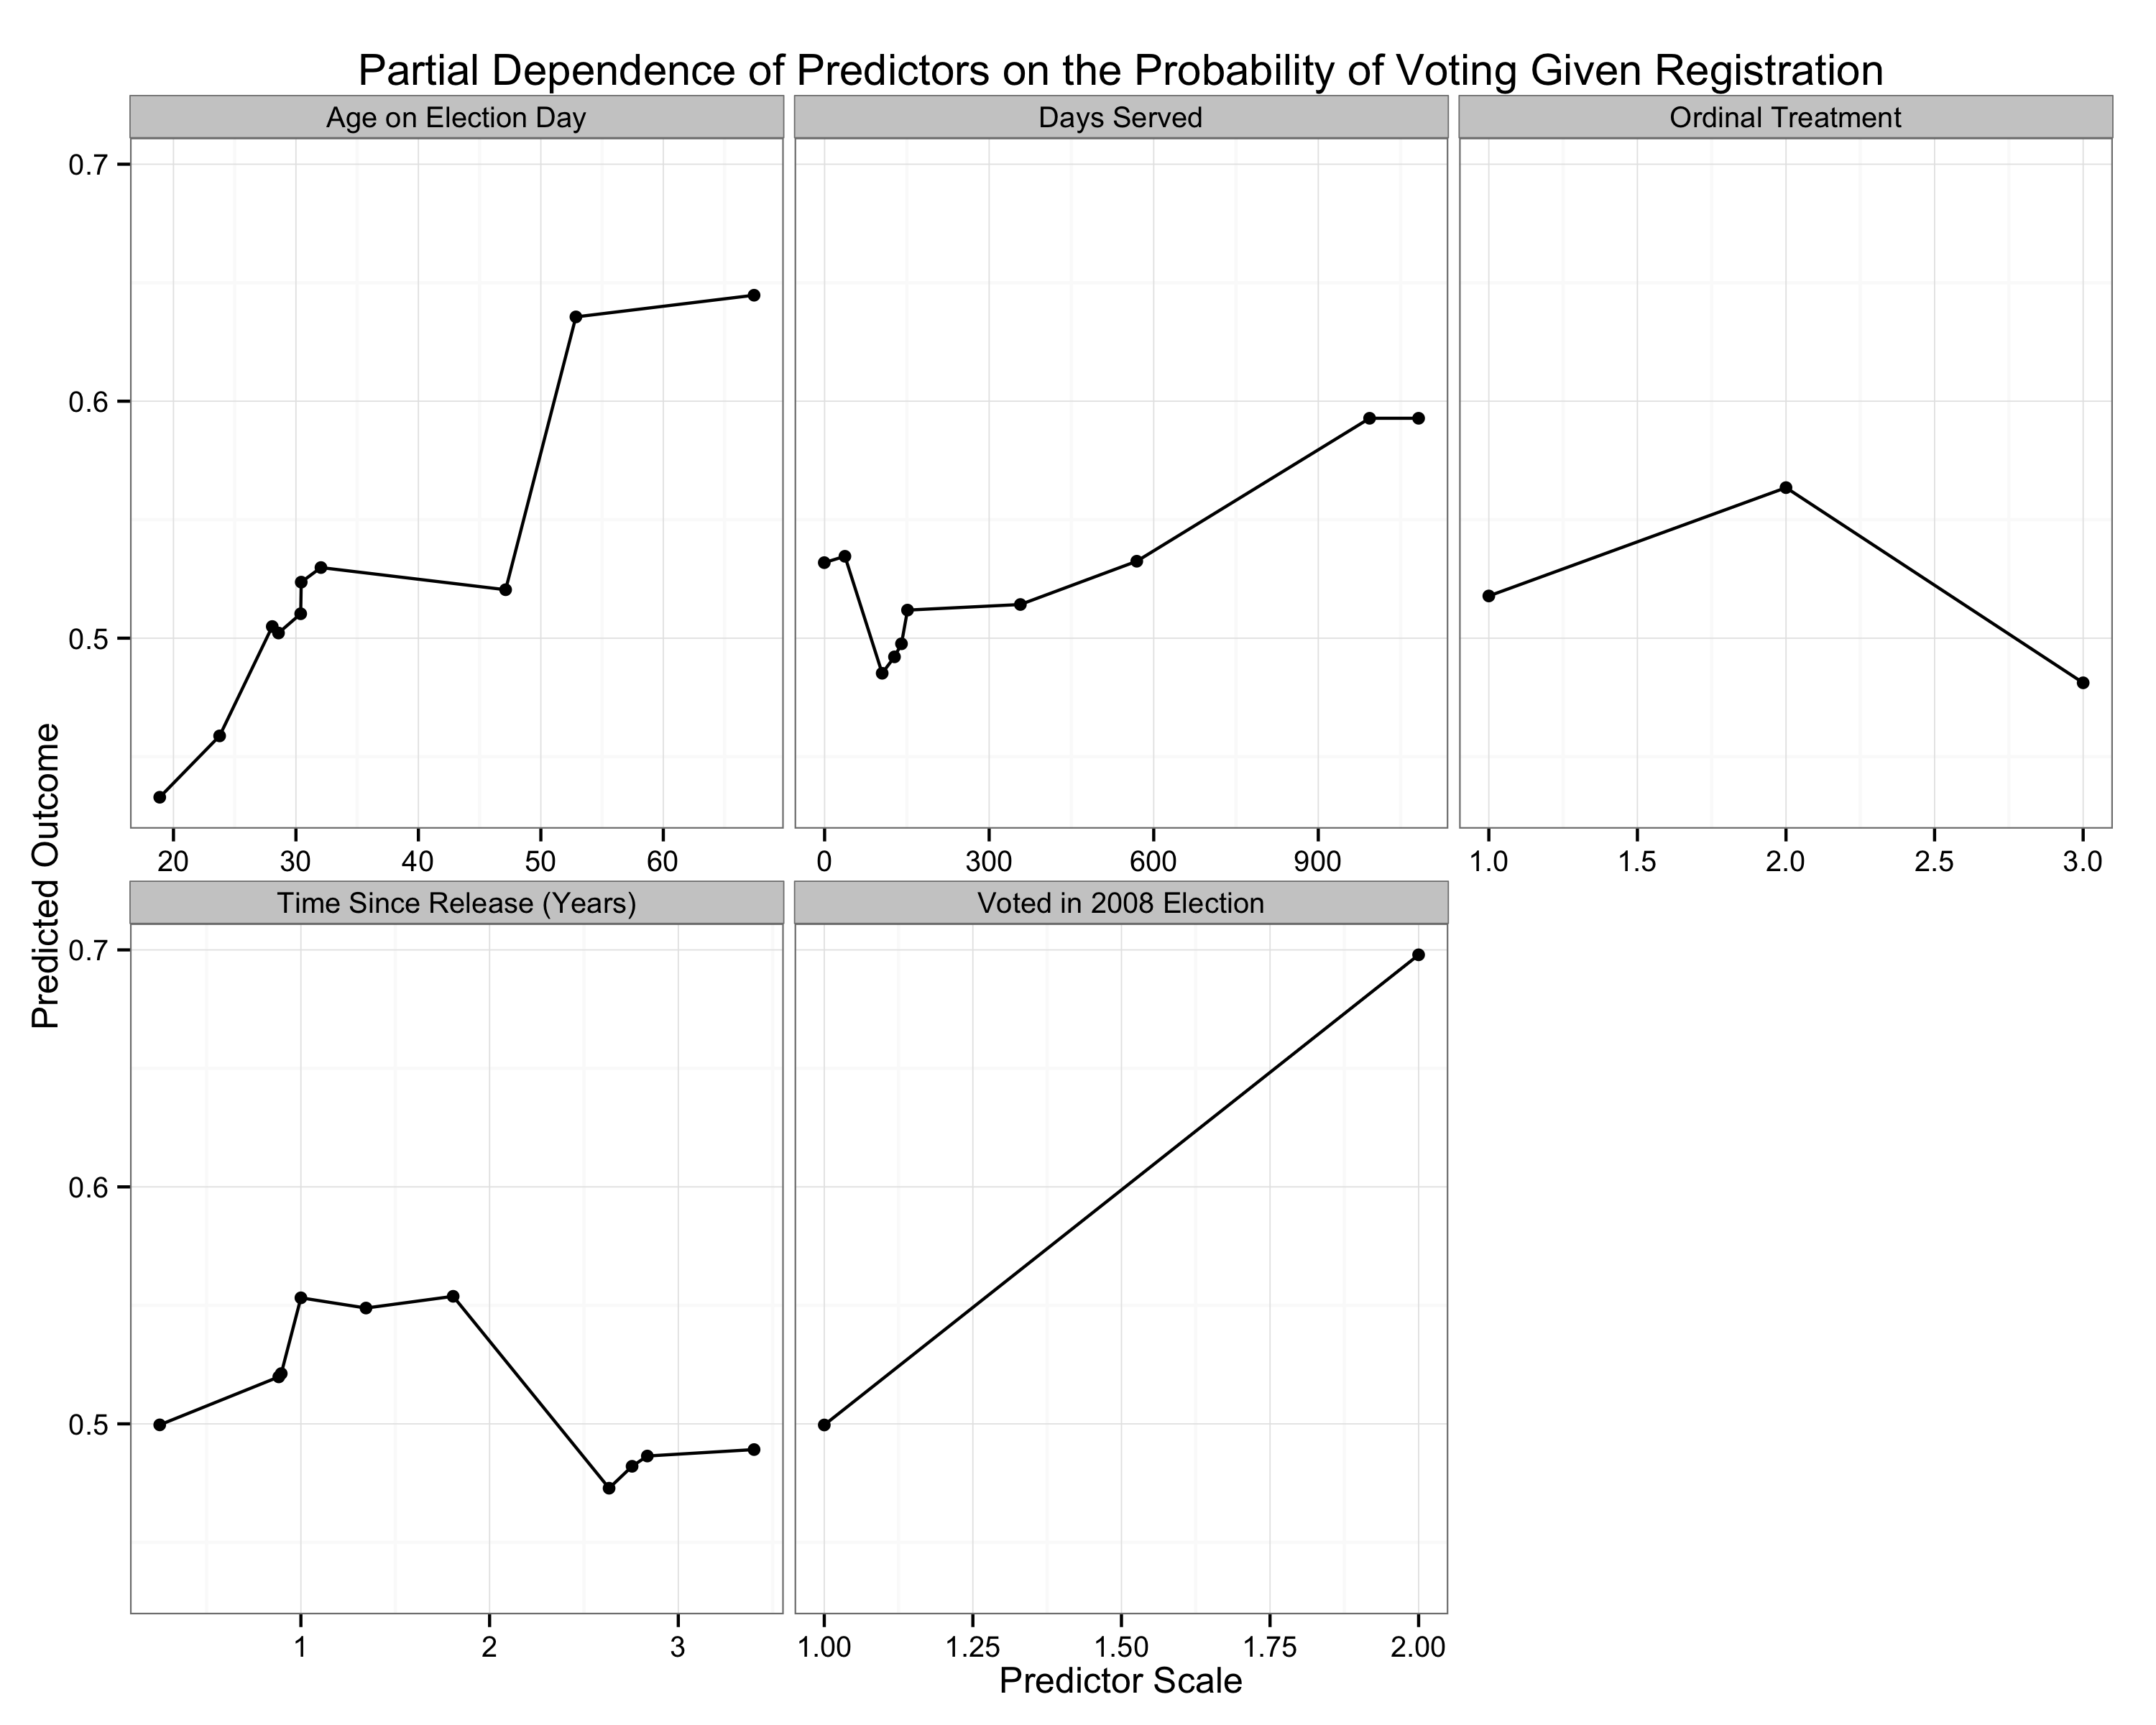
\includegraphics[width=\textwidth]{figures/pd_cond_vote.png}
                \caption{Partial dependence for explanatory variables in the prisoners example.}
                \label{fig:pd_cond_vote}
        \end{subfigure}
        \caption{The partial dependence of the country mean level of latent respect for physical integrity rights by country on World Bank structural adjustment programs, economic sanctions that do not call for increases in respect for physical integrity rights, sanctions which do have such a requirement, whether or not a military regime is in power, the level of executive constraint, the proportion of male youth aged 15-25, contract intensive economy (CIE, a measure of life insurance contracting used by @mousseau2008contracting (from @beck2003economic)), the ratio of trade to gross domestic product (GDP), the "rule of law", the natural log of GDP per capita and population, and judicial independence. Note that the scale of $y$ differs for each sub-plot. The relationship between each predictor and the response is averaged within the joint values of the other predictors conditional on the relationships discovered by the Random Forest.}
        \label{fig:pd}
\end{figure}
